\section{Interpolation Methods}\label{background_interpolation_methods}
    This section focuses on the various statistical methods of interpolating and extrapolating data values at arbitrary points on a grid. These methods vary in their effectiveness on different data sets, however it is important to note that none of these methods take into account data which could be viewed as extremely important in this case. An example of this is the terrain. In section \todo{Fill in this reference} we discuss the effect that canyoning has on air quality readings. This effect is ignored by these models. 

    A further crucial piece of information which needs to be taken into account is that these models do not take into account temporal changes of readings. In order to use our data sets we will have to have a way of ``snapshotting'' data. A choice needs to be made for the length of time each snapshot should be. A suggestion for a rough value is 30 minutes, however experimental results will reveal the best value to use.

    With regards to the models chosen, various possibilities were considered. Due to the fact that various algorithms are similar with minor differences, the decision was made to use only a single algorithm from each ``family''. As such the algorithms chosen to be evaluated are:

    %http://en.wikipedia.org/wiki/Multivariate_interpolation
    \begin{itemize}
        \item Bilinear interpolation
        \item Bicubic interpolation
        \item Natural neighbour interpolation
        \item Barnes interpolation
        \item Nearest neighbour interpolation
        \item Inverse distance weighting interpolation
    \end{itemize}

    These algorithms can be split into two categories, regular grid algorithms and irregular grid algorithms, based on the format of the input data expected. 

    \tdi{Go over all of this. It has been moved around a lot and may not make sense any longer.}

    \tdi{Is this level of detail really required for a lot of these?}

    \subsection{Irregular Grid Algorithms}\label{background_interpolation_methods_irregular_grid}

        These algorithms work with arbitrary data points in that we can specify a single point and calculate the interpolated value for it without being required to calculate an entire grid. They generally all work on regular grids however as these are a subset of irregular grid data points. 

        \subsubsection{Nearest Neighbour}\label{background_interpolation_methods_nearest_neighbour}

            Nearest neighbour interpolation is the simplest interpolation we will see in that it is not really interpolation at all. Instead the value of each point is the value of the closest data point we have. This algorithm can work reasonably well when there is a small amount of variation. However, as the results it produces are discontinuous, it cannot approximate well when there are large differences between adjacent data points~\cite{imageresamplingcomparison}.

            \begin{figure}[H]
                \centering
                \begin{subfigure}{.333\textwidth}
                    \centering
                    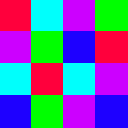
\includegraphics[width=0.9\linewidth]{./images/Nearest_Neighbour_Normal.png}
                    \caption{}
                    \label{fig:example_nearest_neighbour_normal}
                \end{subfigure}%DO NOT REMOVE THIS COMMENT
                \begin{subfigure}{.333\textwidth}
                    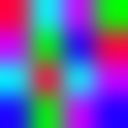
\includegraphics[width=0.9\linewidth]{./images/Nearest_Neighbour_Blur_10px.png}
                    \caption{}
                    \label{fig:example_nearest_neighbour_blur}
                \end{subfigure}%DO NOT REMOVE THIS COMMENT
                \begin{subfigure}{.333\textwidth}
                    \centering
                    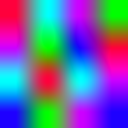
\includegraphics[width=0.9\linewidth]{./images/Nearest_Neighbour_Bicubic.png}
                    \caption{}
                    \label{fig:example_nearest_neighbour_bicubic}
                \end{subfigure}
                \caption{These figures show the similarities between applying a Gaussian Blur to a nearest neighbour interpolation, as seen in figure~\ref{fig:example_nearest_neighbour_blur}, and a bicubic filter, as seen in figure~\ref{fig:example_nearest_neighbour_bicubic}}
                \label{fig:example_nearest_neighbour}
            \end{figure}

            A possible improvement to nearest neighbour is to apply a convolution filter to the data such as that done in figure~\ref{fig:example_nearest_neighbour}. In this figure we originally started with a 4 by 4 pixel image. Using a nearest neighbour algorithm we scaled this up to 128 by 128 pixels as seen in figure~\ref{fig:example_nearest_neighbour_normal}. When we apply a 10 pixel Gaussian Blur, a type of convolution filter, as in figure~\ref{fig:example_nearest_neighbour_blur}, we see that we achieve results similar to that of applying a bicubic interpolation algorithm as in figure~\ref{fig:example_nearest_neighbour_bicubic}.


        \subsubsection{Inverse Distance Weighting}\label{background_interpolation_methods_inverse_distance_weighting}

            The key component of inverse distance weighting (IDW) is the calculation of new parameters as the weighted average of neighbouring parameters. The weighting is calculated as the inverse of the distance from the current point to the neighbour currently being checked and are normalised such that the total weighting is equal to one. Due to the requirement of checking all other points the time complexity of this algorithm, like many other interpolation algorithms, is $O(n^{2})$. However it is possible to reduce this by some constant factor by imposing a maximum radius on all calculations. 

            The general formula for calculating the value, $V$, at a point $X_{i}$, given samples $S$, where $f(S_{i})$ is the value of sample $S$, is:

            \begin{align*}
                V = \sum_{i=1}^{N}{f(S_{i})\frac{w_{i}(X_{i})}{\sum_{j=0}^{N}{w_{j}(X_{j})}}},
            \end{align*}

            where 

            \begin{align*}
                w_{i}(x) = \frac{1}{d(x,S_{i})^{p}}
            \end{align*}

            is a weighting function with $d(X_{1},X_{2})$ being a distance metric between points $X_{1}$ and $X_{2}$, and $p$ is the power parameter, which controls the rate of change at which distances affect the weighting.

            \begin{figure}[H]
                \centering
                \begin{subfigure}{.5\textwidth}
                    \centering
                    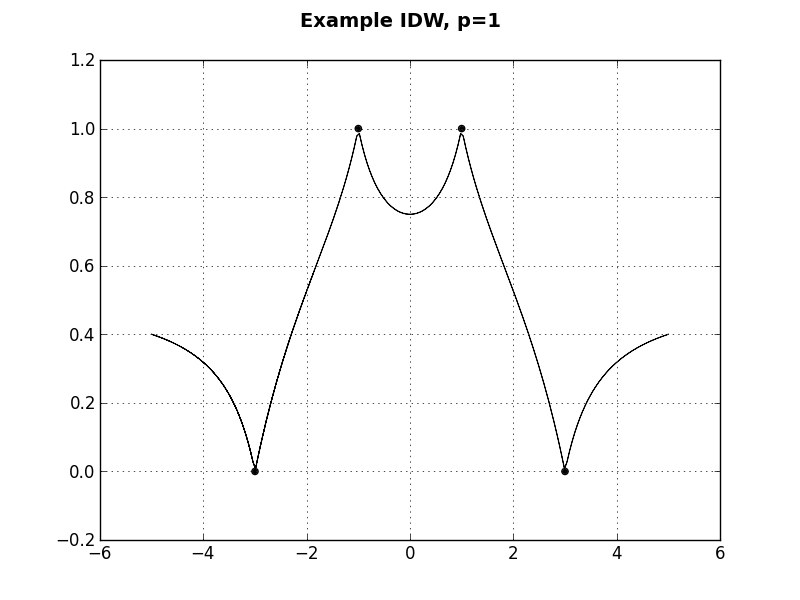
\includegraphics[width=\linewidth]{./images/IDWPF1.png}
                    \caption{}
                    \label{fig:example_idw_p1}
                \end{subfigure}%DO NOT REMOVE THIS COMMENT
                \begin{subfigure}{.5\textwidth}
                    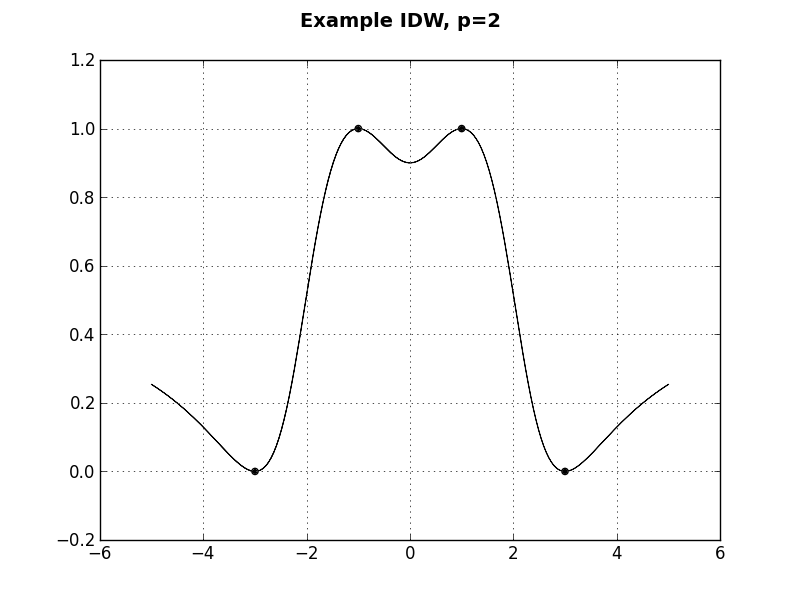
\includegraphics[width=\linewidth]{./images/IDWPF2.png}
                    \caption{}
                    \label{fig:example_idw_p2}
                \end{subfigure}
                \begin{subfigure}{.5\textwidth}
                    \centering
                    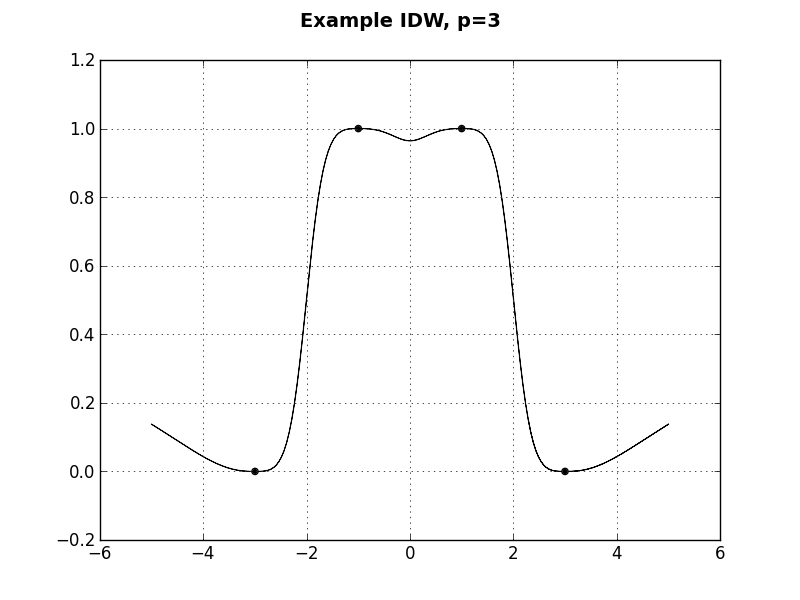
\includegraphics[width=\linewidth]{./images/IDWPF3.png}
                    \caption{}
                    \label{fig:example_idw_p3}
                \end{subfigure}%DO NOT REMOVE THIS COMMENT
                \begin{subfigure}{.5\textwidth}
                    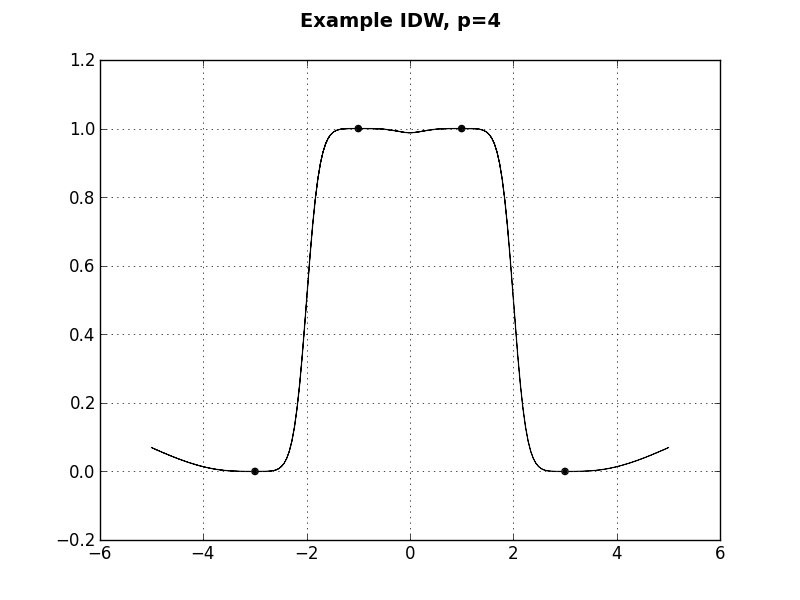
\includegraphics[width=\linewidth]{./images/IDWPF4.png}
                    \caption{}
                    \label{fig:example_idw_p4}
                \end{subfigure}
                \caption{These two figures show the IDW algorithm in one dimension at points -3,-1,1 and 3 where the values are 0,1,1 and 0 respectively. Figures~\ref{fig:example_idw_p1},~\ref{fig:example_idw_p2},~\ref{fig:example_idw_p3} and ~\ref{fig:example_idw_p4} have power parameters of 1,2,3 and 4 respectively.}
                \label{fig:example_idw}
            \end{figure}

            As we can see in figure~\ref{fig:example_idw_p1} IDW's dependence on the surrounding values causes interesting effects. Between the x values of -1 and 1 we can see a local minima in the graph. This is due to the fact that the values at -3 and 3 are lower and are taken into account. A way of mitigating this effect is to increase the power parameter as has been done in figures~\ref{fig:example_idw_p1},~\ref{fig:example_idw_p2},~\ref{fig:example_idw_p3} and ~\ref{fig:example_idw_p4}. It should be noted, however, that as the p factor goes to infinity, the IDW algorithm approaches the nearest neighbour algorithm. 

            A further example of this effect is figure~\ref{fig:example_idw_distance}, which has the extreme values further away, causing the local minima to be less pronounced.

            \centerimage{.5\textwidth}{./images/IDW_distance.png}{In this figure the two extreme points have been moved further from zero by a value of one, in order to demonstrate their effect on the value at zero decreasing compared to figure~\ref{fig:example_idw_p2}}{fig:example_idw_distance}


    \subsection{Regular Grid Algorithms}\label{background_interpolation_methods_regulargrid}

        Regular grid algorithms require the known data points to be on a regular grid and can not easily only calculate the interpolated value of a single point. This can be achieved with irregular data by making the grid sufficiently large and ``snapping'' data points to it.

        \subsubsection{Bilinear}\label{background_interpolation_methods_bilinear}

            Bilinear interpolation, is the simplest of the grid interpolation algorithms which will be evaluated. The algorithm is the two dimensional equivalent of linear interpolation, and works by evaluating the linear interpolation in both the x and y directions and combining them. Essentially this calculates each pixel as a weighted average of the 4 nearest pixels.

            The main disadvantage of bilinear interpolation is that if there is an outlier point nearby then this has a large effect on interpolated points. It also has the disadvantage that it cannot extrapolate any information. All points to be interpolated must be inside the convex hull of the known points.


        \subsubsection{Bicubic}\label{background_interpolation_methods_bicubic}

            Bicubic interpolation, a popular algorithm in image resampling, is essentially an improved version of bilinear interpolation, when applied to images. As a cubic Hermite spline~\cite{practicalguidesplines}, the output is smoother than linear interpolation, as we can see in figure~\ref{fig:bicubic_vs_bilinear}. The bicubic algorithm achieves this by taking into account the 16 points surrounding the point to be interpolated rather than just 4. 

            \begin{figure}[H]
                \centering
                \begin{subfigure}{.5\textwidth}
                    \centering
                    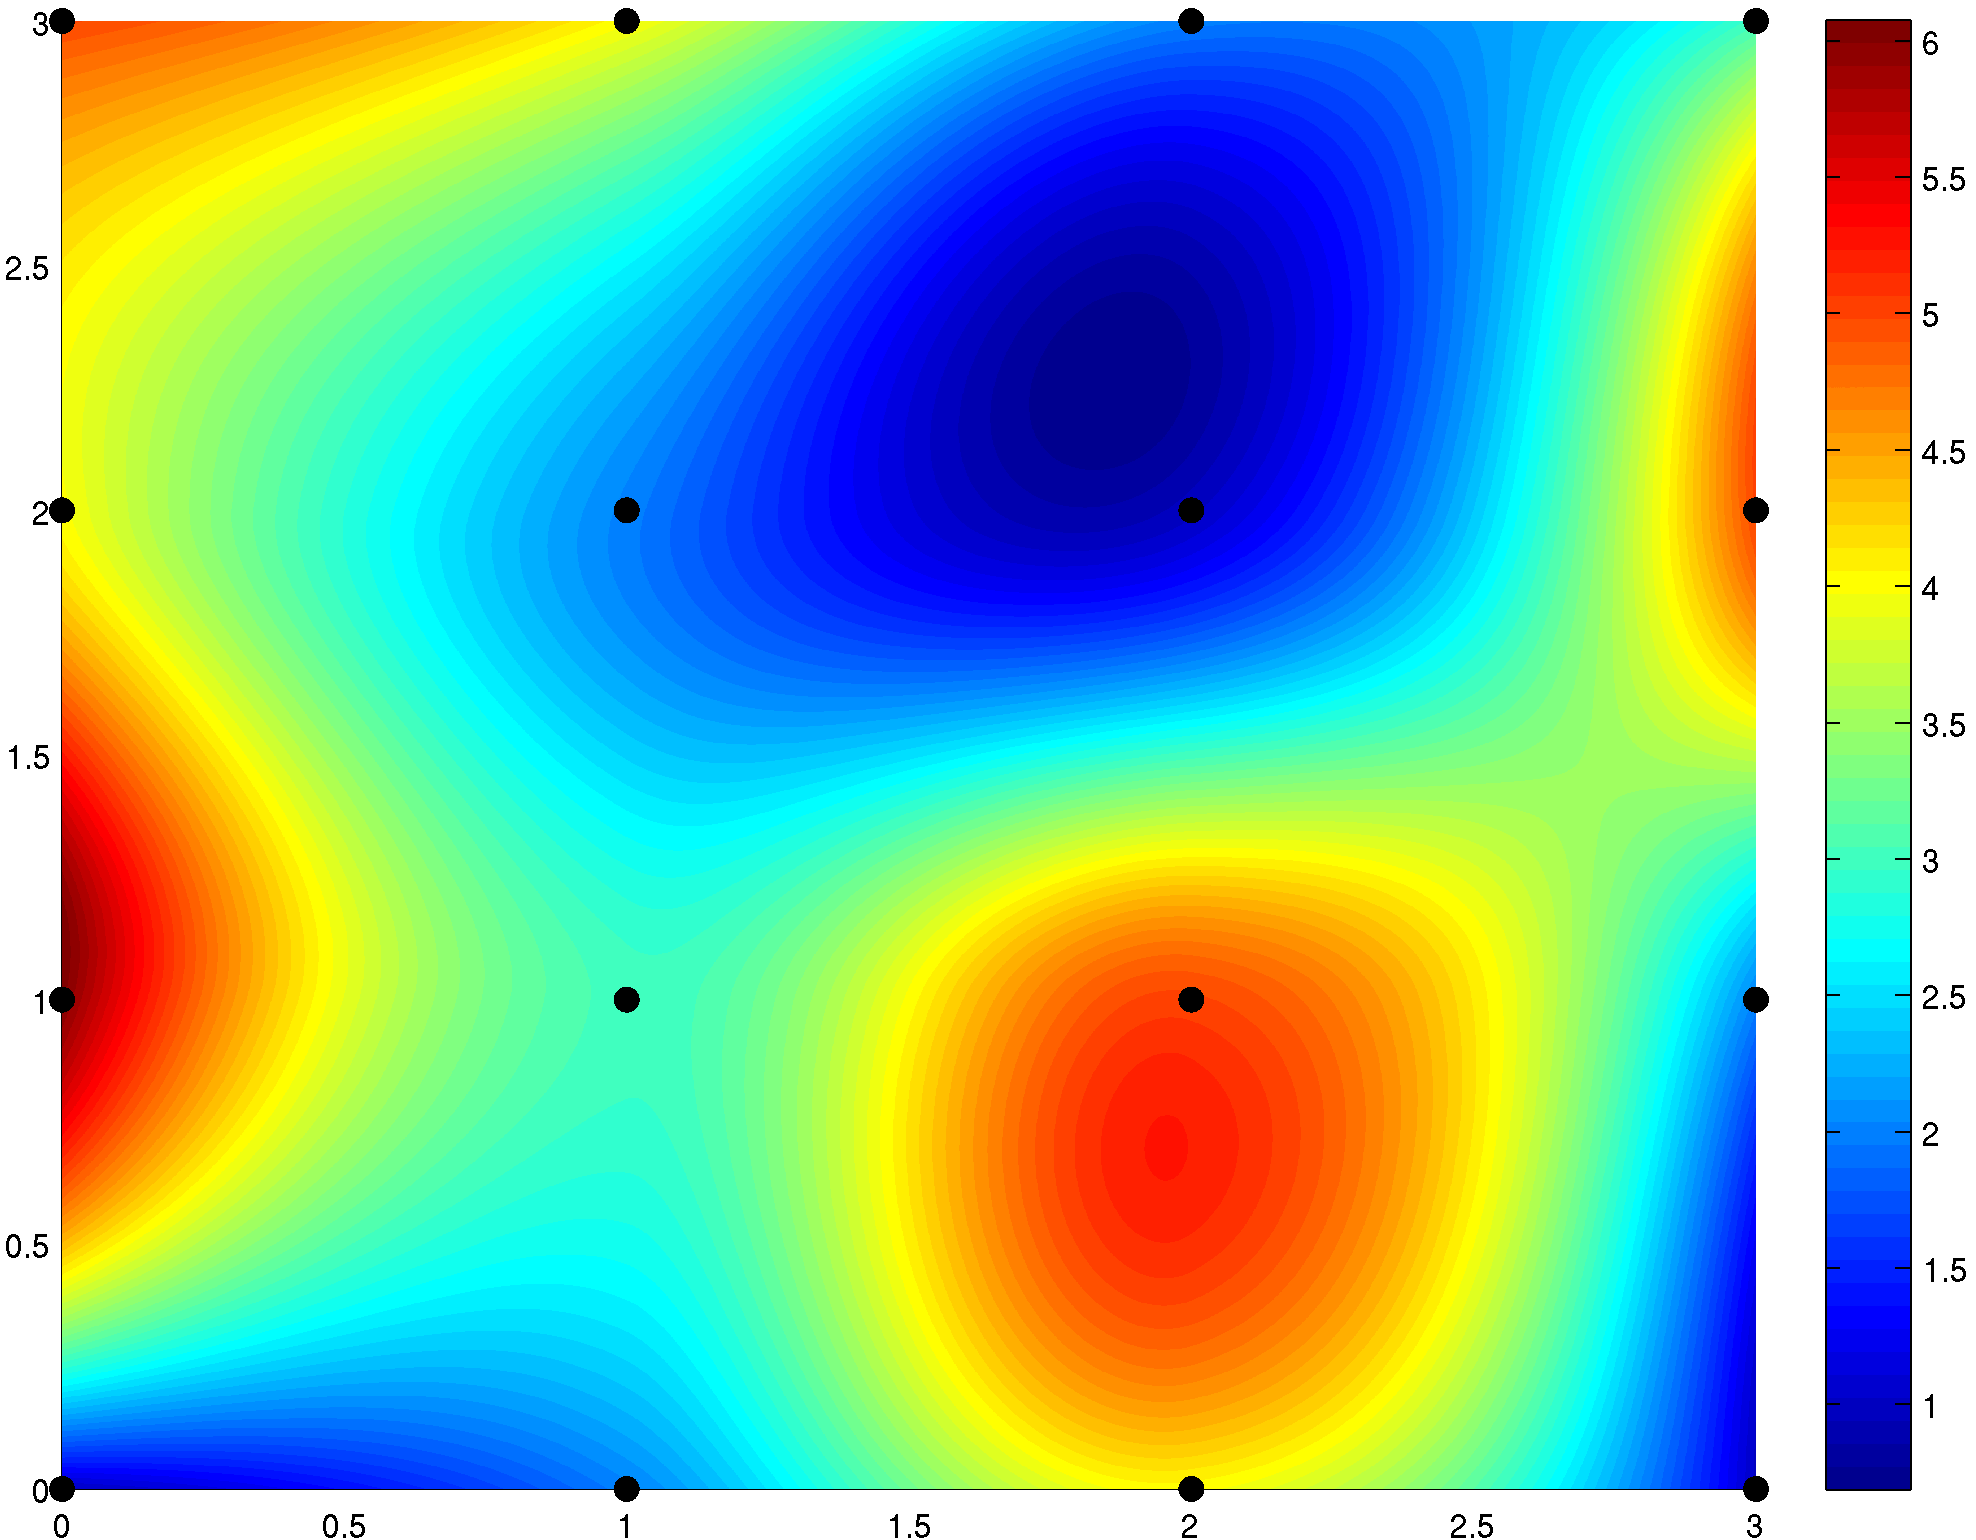
\includegraphics[width=0.9\linewidth]{./images/Bicubic_Interpolation_Example.png}
                    \caption{}
                    \label{fig:example_bicubic}
                \end{subfigure}%DO NOT REMOVE THIS COMMENT
                \begin{subfigure}{.5\textwidth}
                    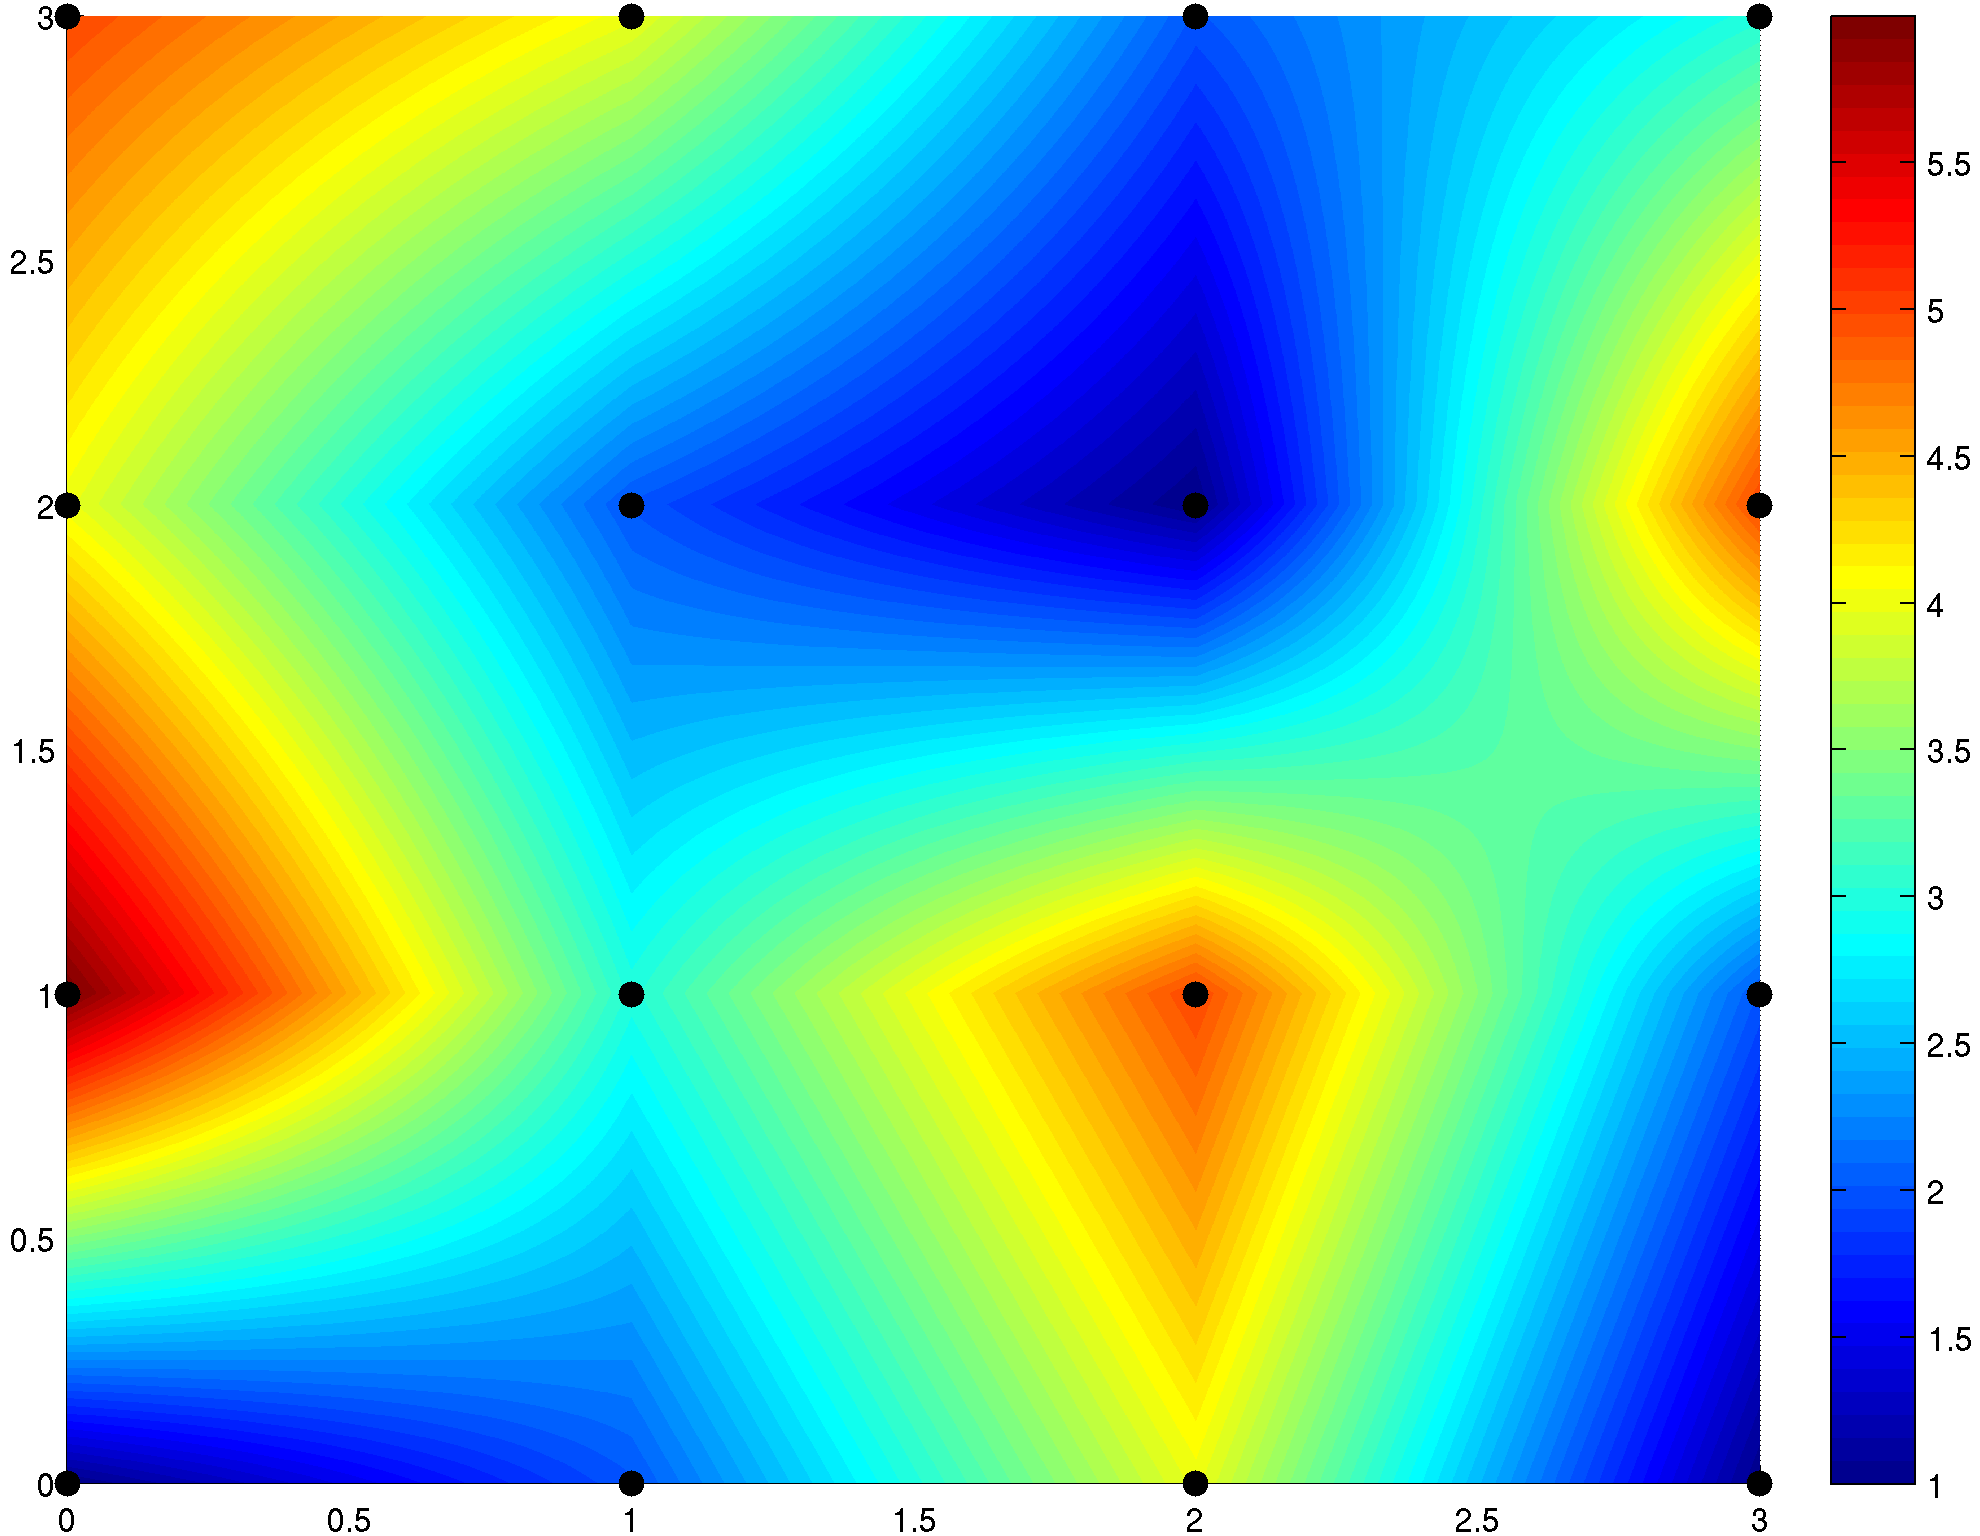
\includegraphics[width=0.9\linewidth]{./images/Bilinear_Interpolation_Example.png}
                    \caption{}
                    \label{fig:example_bilinear}
                \end{subfigure}
                \caption{These examples, created by Wikipedia user \emph{Berland}, shows the difference between bicubic interpolation, figure~\ref{fig:example_bicubic}, and bilinear interpolation, figure~\ref{fig:example_bilinear}, on the same dataset.}
                \label{fig:bicubic_vs_bilinear}
            \end{figure}

            The algorithm for bicubic interpolation is relatively simple, with the result being given by the calculation:

            \begin{align*}
                p(x,y) = \sum_{i=0}^{3}{\sum_{j=0}^{3}{a_{ij}x^{i}y^{j}}},
            \end{align*}

            with the values of $a_{ij}$ being determined by solving a system of linear equations~\cite{bicubicorigins}.

            As with the bilinear interpolation algorithm, we cannot extrapolate, only interpolate. 

        \subsubsection{Natural Neighbour}\label{background_interpolation_methods_natural_neighbour}

            Natural neighbour interpolation is based on Voronoi tessellation~\cite{multivariatedata}. The basic method is very similar to that of IDW in that the basic form of the equation is:

            \begin{align*}
                G(x,y) = \sum_{i=1}^{n}{w_{i}f(x_{i},y_{i})}, 
            \end{align*}

            where $w_{i}$ is the weighting factor and $f(x_{i},y_{i})$ is the value at known point $(x_{i},y_{i})$. The main difference between natural neighbour and IDW is the method used to calculate the weighing. In natural neighbour the weighting is calculated as the ratio of area of the new region that originally belonged to the current known point in a Voronoi diagram. As such all weightings sum to one, which ensures that the original values do not change. An example of this can be seen in figure~\ref{fig:natural_neighbour}.

            \begin{figure}[H]
                \begin{center}
                    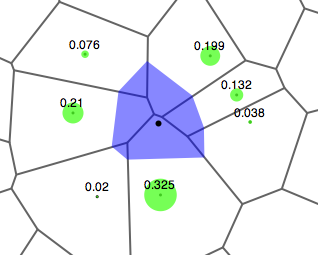
\includegraphics[scale=0.66]{./images/Natural_Neighbour.png}
                    \caption{An example of how the weighing in natural neighbour is calculated. This figure was created by Wikipedia user \emph{Markluffel}.}
                    \label{fig:natural_neighbour}
                \end{center}
            \end{figure}

        \subsubsection{Barnes}\label{background_interpolation_methods_barnes}

            Barnes interpolation uses a multi-pass approach to determine the new data points. The method has found success in calculating air pressure across the United States, providing results similar to careful analysis, however it depends on the data points be reasonably uniform~\cite{barnesinterpolation}.

            The algorithm works by calculating a simple distance weighted interpolation as the first result, and then iterating multiple times using a calculated error field to reduce the errors in the output. 

            One important factor in Barnes interpolation is the fact that it depends on several constants. These constants depend on the type of data being interpolated and the nature of the measurements, including the density of the measurements. As such, determining these constants is a key part of using this algorithm for interpolation. One advantage of this approach, is that we can iterate over our data set and fit it to the known measurements in order to make sure it is as accurate as possible. With this method however, we lose test data points and so cannot validate it. Experiments using this algorithm have used similar mechanisms and shown success~\cite{pmconcentrationmaps}.

            The algorithm for Barnes interpolation is as follows.

            For the first pass each known point is assigned a weight using the formula: 

            \begin{align*}
                W_{i} &= e^{-(d/R^{2})}
            \end{align*}
            
            where d is the distance between the known point and the current point to be interpolated, and R is the radius of influence. Using this weight, the initial guess of the grid points is calculated as: 
            
            \begin{align*}
                X_{g} &= \frac{\sum_{i}{W_{i}X_{i}}}{\sum_{i}{W_{i}}}
            \end{align*}

            At this point we begin our successive passes. These are defined as:

            \begin{align*}
                X'_{g} &= X_{g} + \frac{\sum_{i}{W'_{i}E_{i}}}{\sum_{i}{W'_{i}}}
            \end{align*}

            where $E_{k}$ is the difference between the estimated value and the actual value at a known point $k$ and $W'_{i}$ is defined as:

            \begin{align*}
                W'_{i} &= e^{-(d/\Gamma R)^{2}}
            \end{align*}

            with $\Gamma$ as a convergence parameter normally set in the range 0.2-0.3.


